% =====================================================================
%  Laborbericht  –  Versuch 9: Anlauf- und Bremsverfahren
%  Ostfalia Hochschule, Labor für elektrische Antriebe
%  Übersetzen:  pdflatex bericht.tex  (2x, wegen Verzeichnissen)
%  Alle Zahlenwerte \W... stammen aus werte.tex (erzeugt von
%  ../auswertung/auswertung.py). Nach Änderungen an den Daten einfach
%  das Skript erneut ausführen und den Bericht neu übersetzen.
% =====================================================================
\documentclass[11pt,a4paper]{article}
\usepackage[utf8]{inputenc}
\usepackage[T1]{fontenc}
\usepackage[ngerman]{babel}
\usepackage{lmodern}
\usepackage{microtype}
\usepackage[a4paper,left=2.5cm,right=2.5cm,top=2.8cm,bottom=2.6cm,headheight=28pt]{geometry}
\usepackage{amsmath,amssymb}
\usepackage[locale=DE,per-mode=symbol]{siunitx}
\usepackage{graphicx}
\usepackage{booktabs,tabularx,array,multirow}
\usepackage{float}
\usepackage{longtable}
\usepackage{caption}
\captionsetup{font=small,labelfont=bf}
\usepackage{fancyhdr}
\usepackage{enumitem}
\setlist{itemsep=2pt,topsep=4pt}
\usepackage{xcolor}
\usepackage[colorlinks=true,linkcolor=black,citecolor=black,urlcolor=blue!50!black]{hyperref}
\usepackage{tcolorbox}

\graphicspath{{abbildungen/}}
% automatisch erzeugt von auswertung/auswertung.py
\newcommand{\WJStahl}{0{,}3711}
\newcommand{\WJAlu}{0{,}1277}
\newcommand{\WJVorb}{0{,}3745}
\newcommand{\WdtBsp}{42{,}6}
\newcommand{\WtHDA}{1{,}20}
\newcommand{\WtHDB}{1{,}29}
\newcommand{\WtHDC}{1{,}40}
\newcommand{\WtHYA}{3{,}62}
\newcommand{\WtHYB}{3{,}92}
\newcommand{\WtHYC}{4{,}24}
\newcommand{\WdirektIeins}{50{,}66}
\newcommand{\WdirektUnull}{405}
\newcommand{\WdirektUeins}{388}
\newcommand{\WdirektPeins}{17896}
\newcommand{\WdirektQeins}{56162}
\newcommand{\Wdirektnend}{1499}
\newcommand{\WdirektIend}{4{,}58}
\newcommand{\WdirektPend}{1747}
\newcommand{\WdirektQend}{5175}
\newcommand{\Wdirekttneunacht}{1{,}14}
\newcommand{\Wdirektteinsvierfuenfnull}{1{,}10}
\newcommand{\WdirektE}{14509}
\newcommand{\WdirektdU}{4{,}3}
\newcommand{\WdirektIfak}{11{,}0}
\newcommand{\WdirektIN}{7{,}6}
\newcommand{\WfruehIeins}{15{,}51}
\newcommand{\WfruehUnull}{405}
\newcommand{\WfruehUeins}{400}
\newcommand{\WfruehPeins}{6685}
\newcommand{\WfruehQeins}{17788}
\newcommand{\Wfruehnend}{1497}
\newcommand{\WfruehIend}{4{,}59}
\newcommand{\WfruehPend}{1760}
\newcommand{\WfruehQend}{5173}
\newcommand{\Wfruehtneunacht}{2{,}65}
\newcommand{\Wfruehteinsvierfuenfnull}{2{,}62}
\newcommand{\WfruehE}{15389}
\newcommand{\WfruehdU}{1{,}2}
\newcommand{\WfruehIfak}{3{,}4}
\newcommand{\WfruehIN}{2{,}3}
\newcommand{\Wfruehtum}{1{,}91}
\newcommand{\Wfruehnum}{724}
\newcommand{\Wfruehpause}{0{,}16}
\newcommand{\WfruehIzwei}{45{,}91}
\newcommand{\WfruehUzwei}{384}
\newcommand{\WfruehPzwei}{20422}
\newcommand{\WfruehdUzwei}{5{,}1}
\newcommand{\WrichtigIeins}{15{,}51}
\newcommand{\WrichtigUnull}{405}
\newcommand{\WrichtigUeins}{400}
\newcommand{\WrichtigPeins}{5635}
\newcommand{\WrichtigQeins}{17779}
\newcommand{\Wrichtignend}{1497}
\newcommand{\WrichtigIend}{4{,}57}
\newcommand{\WrichtigPend}{1755}
\newcommand{\WrichtigQend}{5162}
\newcommand{\Wrichtigtneunacht}{3{,}86}
\newcommand{\Wrichtigteinsvierfuenfnull}{3{,}82}
\newcommand{\WrichtigE}{15754}
\newcommand{\WrichtigdU}{1{,}3}
\newcommand{\WrichtigIfak}{3{,}4}
\newcommand{\WrichtigIN}{2{,}3}
\newcommand{\Wrichtigtum}{3{,}60}
\newcommand{\Wrichtignum}{1443}
\newcommand{\Wrichtigpause}{0{,}14}
\newcommand{\WrichtigIzwei}{42{,}25}
\newcommand{\WrichtigUzwei}{402}
\newcommand{\WrichtigPzwei}{11284}
\newcommand{\WrichtigdUzwei}{0{,}9}
\newcommand{\WfalschIeins}{15{,}71}
\newcommand{\WfalschUnull}{405}
\newcommand{\WfalschUeins}{400}
\newcommand{\WfalschPeins}{5622}
\newcommand{\WfalschQeins}{18202}
\newcommand{\Wfalschnend}{1498}
\newcommand{\WfalschIend}{4{,}58}
\newcommand{\WfalschPend}{1781}
\newcommand{\WfalschQend}{5172}
\newcommand{\Wfalschtneunacht}{3{,}90}
\newcommand{\Wfalschteinsvierfuenfnull}{3{,}59}
\newcommand{\WfalschE}{15842}
\newcommand{\WfalschdU}{1{,}3}
\newcommand{\WfalschIfak}{3{,}4}
\newcommand{\WfalschIN}{2{,}4}
\newcommand{\Wfalschtum}{3{,}62}
\newcommand{\Wfalschnum}{1453}
\newcommand{\Wfalschpause}{0{,}15}
\newcommand{\WfalschIzwei}{50{,}91}
\newcommand{\WfalschUzwei}{401}
\newcommand{\WfalschPzwei}{19180}
\newcommand{\WfalschdUzwei}{1{,}0}
\newcommand{\WtHYum}{3{,}87}
\newcommand{\WdirektMBmittel}{52{,}7}
\newcommand{\WfruehMBmittel}{14{,}8}
\newcommand{\WrichtigMBmittel}{15{,}8}
\newcommand{\WfalschMBmittel}{15{,}9}
\newcommand{\WMkennDmittel}{48{,}8}
\newcommand{\WMkennYmittel}{16{,}1}
\newcommand{\WEkin}{2268}
\newcommand{\Wfedernnull}{1801}
\newcommand{\WfedertB}{0{,}88}
\newcommand{\Wfederts}{0{,}12}
\newcommand{\WfederMmit}{31{,}7}
\newcommand{\WfederMmax}{32{,}0}
\newcommand{\WfederUzkmax}{583}
\newcommand{\WfederErb}{0}
\newcommand{\Wfederverz}{2047}
\newcommand{\Wfedernullnnull}{1801}
\newcommand{\WfedernulltB}{0{,}90}
\newcommand{\Wfedernullts}{0{,}12}
\newcommand{\WfedernullMmit}{30{,}8}
\newcommand{\WfedernullMmax}{31{,}3}
\newcommand{\WfedernullUzkmax}{583}
\newcommand{\WfedernullErb}{0}
\newcommand{\Wfedernullverz}{1996}
\newcommand{\WdclnI}{1773}
\newcommand{\WdclIdcB}{14{,}1}
\newcommand{\WdclIeffB}{9{,}4}
\newcommand{\WdcltI}{1{,}03}
\newcommand{\WdcltnachI}{5{,}17}
\newcommand{\Wdclnnull}{1801}
\newcommand{\WdcltB}{6{,}20}
\newcommand{\Wdclts}{0{,}40}
\newcommand{\WdclMmit}{4{,}6}
\newcommand{\WdclMmax}{21{,}4}
\newcommand{\WdclUzkmax}{595}
\newcommand{\WdclErb}{0}
\newcommand{\Wdclverz}{290}
\newcommand{\WdcmnI}{1774}
\newcommand{\WdcmIdcB}{20{,}5}
\newcommand{\WdcmIeffB}{13{,}7}
\newcommand{\WdcmtI}{1{,}02}
\newcommand{\WdcmtnachI}{2{,}43}
\newcommand{\Wdcmnnull}{1801}
\newcommand{\WdcmtB}{3{,}45}
\newcommand{\Wdcmts}{0{,}41}
\newcommand{\WdcmMmit}{9{,}7}
\newcommand{\WdcmMmax}{33{,}9}
\newcommand{\WdcmUzkmax}{596}
\newcommand{\WdcmErb}{0}
\newcommand{\Wdcmverz}{521}
\newcommand{\WdcsnI}{1774}
\newcommand{\WdcsIdcB}{32{,}8}
\newcommand{\WdcsIeffB}{21{,}9}
\newcommand{\WdcstI}{1{,}03}
\newcommand{\WdcstnachI}{0{,}95}
\newcommand{\Wdcsnnull}{1801}
\newcommand{\WdcstB}{1{,}98}
\newcommand{\Wdcsts}{0{,}42}
\newcommand{\WdcsMmit}{25{,}5}
\newcommand{\WdcsMmax}{57{,}5}
\newcommand{\WdcsUzkmax}{596}
\newcommand{\WdcsErb}{0}
\newcommand{\Wdcsverz}{929}
\newcommand{\Wgenohnennull}{1801}
\newcommand{\WgenohnetB}{8{,}49}
\newcommand{\Wgenohnets}{0{,}09}
\newcommand{\WgenohneMmit}{2{,}9}
\newcommand{\WgenohneMmax}{19{,}6}
\newcommand{\WgenohneUzkmax}{815}
\newcommand{\WgenohneErb}{0}
\newcommand{\Wgenohneverz}{211}
\newcommand{\Wgenlnnull}{1801}
\newcommand{\WgenltB}{10{,}12}
\newcommand{\Wgenlts}{0{,}14}
\newcommand{\WgenlMmit}{2{,}4}
\newcommand{\WgenlMmax}{2{,}8}
\newcommand{\WgenlUzkmax}{724}
\newcommand{\WgenlErb}{512}
\newcommand{\Wgenlverz}{177}
\newcommand{\Wgenmnnull}{1801}
\newcommand{\WgenmtB}{5{,}13}
\newcommand{\Wgenmts}{0{,}10}
\newcommand{\WgenmMmit}{4{,}8}
\newcommand{\WgenmMmax}{5{,}8}
\newcommand{\WgenmUzkmax}{724}
\newcommand{\WgenmErb}{1365}
\newcommand{\Wgenmverz}{349}
\newcommand{\Wgensnnull}{1801}
\newcommand{\WgenstB}{0{,}87}
\newcommand{\Wgensts}{0{,}06}
\newcommand{\WgensMmit}{29{,}6}
\newcommand{\WgensMmax}{39{,}2}
\newcommand{\WgensUzkmax}{723}
\newcommand{\WgensErb}{1821}
\newcommand{\Wgensverz}{2061}
\newcommand{\WRb}{28}
\newcommand{\WPRbmax}{7760}
\newcommand{\WgensErbAnteil}{80}


\newcommand{\upm}{\si{\per\minute}}
\newcommand{\versuch}{Versuch 9: Anlauf- und Bremsverfahren}

% Antwortbox für die Fragen der Versuchsanleitung
\newtcolorbox{antwort}[1]{colback=blue!3,colframe=blue!45!black,
  fonttitle=\bfseries\small,title={#1},boxrule=0.6pt,arc=1mm,left=4pt,right=4pt}

\pagestyle{fancy}
\fancyhf{}
\fancyhead[L]{Labor für elektrische Antriebe}
\fancyhead[R]{\versuch}
\fancyfoot[L]{Laborbericht}
\fancyfoot[R]{Seite \thepage}
\renewcommand{\headrulewidth}{0.4pt}
\renewcommand{\footrulewidth}{0.4pt}

\begin{document}

% ------------------------------------------------------------ Deckblatt
\begin{titlepage}
\thispagestyle{empty}
\begin{center}
{\large Ostfalia Hochschule für angewandte Wissenschaften}\\[2pt]
{\large Fakultät Elektrotechnik}\\[1.2cm]
{\Large\bfseries Labor für elektrische Antriebe}\\[1.6cm]
\rule{\textwidth}{0.8pt}\\[0.4cm]
{\huge\bfseries Laborbericht}\\[0.4cm]
{\LARGE Versuch 9: Anlauf- und Bremsverfahren}\\[0.2cm]
{\large von Asynchronmaschinen}\\[0.3cm]
\rule{\textwidth}{0.8pt}\\[1.6cm]
\end{center}

\renewcommand{\arraystretch}{1.9}
\begin{tabularx}{\textwidth}{@{}l X l l@{}}
Betreuer: & Prof.\ Dr.-Ing.\ Karl-Dieter Tieste, Dipl.-Ing.\ Roland Hippel & & \\[6pt]
Teilnehmer 1: & \hrulefill & Matr.-Nr.: & \rule{2.4cm}{0.4pt}\\
Teilnehmer 2: & \hrulefill & Matr.-Nr.: & \rule{2.4cm}{0.4pt}\\
Teilnehmer 3: & \hrulefill & Matr.-Nr.: & \rule{2.4cm}{0.4pt}\\[6pt]
Gruppe: & \hrulefill & & \\
Versuchsdatum: & \hrulefill & & \\
Abgabedatum: & \hrulefill & & \\
\end{tabularx}
\renewcommand{\arraystretch}{1}
\vfill
\begin{center}\small
Grundlage: Versuchsanleitung V9 „Anlauf- und Bremsverfahren“\\ Version 0.9 vom 08.10.2026
\end{center}
\end{titlepage}

\tableofcontents
\newpage

% =====================================================================
\section{Einleitung und Ziel des Versuchs}
% =====================================================================
Drehstrom-Asynchronmaschinen (ASM) mit Käfigläufer sind die am häufigsten
eingesetzten elektrischen Antriebe. Beim direkten Einschalten nehmen sie einen
Anlaufstrom auf, der ein Vielfaches des Nennstroms beträgt und das speisende Netz
belastet. Beim Abschalten laufen sie dagegen ohne Bremse wegen der gespeicherten
kinetischen Energie lange nach.

Ziel des Versuchs ist es,
\begin{itemize}
  \item den \textbf{direkten Dreieckanlauf} mit dem \textbf{Stern-Dreieck-Anlauf}
        (zu früh und richtig umgeschaltet) messtechnisch zu vergleichen,
  \item die Hochlaufzeit einer ASM mit Schwungmasse vorab aus der
        Drehmoment-Drehzahl-Kennlinie zu \textbf{berechnen} und mit der Messung zu vergleichen,
  \item die Bremsverfahren \textbf{Federkraftbremse}, \textbf{Gleichstrombremsung} sowie
        \textbf{generatorisches Bremsen mit und ohne Bremswiderstand} zu untersuchen und
  \item aus den gemessenen Drehzahlverläufen die wirkenden Beschleunigungs- bzw.\ Bremsmomente zu bestimmen.
\end{itemize}

% =====================================================================
\section{Theoretische Grundlagen}
% =====================================================================
\subsection{Anlaufverhalten der Asynchronmaschine}
Im Stillstand ist der Schlupf $s = 1$. Die ASM verhält sich dann wie ein
Transformator mit kurzgeschlossener Sekundärwicklung: Wirksam ist nur die kleine
Kurzschlussimpedanz, sodass der Anlaufstrom typischerweise das 5- bis 8-fache des
Nennstroms erreicht. Dieser Strom ist überwiegend induktiv (kleiner
Leistungsfaktor). Mit steigender Drehzahl sinkt der Schlupf, die wirksame
Impedanz steigt und der Strom geht auf den Last- bzw.\ Leerlaufstrom zurück.

\subsection{Belastung des Netzes und Spannungseinbruch}
Der Anlaufstrom $\underline I_1$ fließt über die Kurzschlussimpedanz
$\underline Z_k = R_k + \mathrm{j}X_k$ des Netztransformators und der Zuleitungen.
Nach dem Kapp'schen Dreieck gilt für den Spannungsabfall näherungsweise
\begin{equation}
  \Delta U \approx I_1\,(R_k\cos\varphi + X_k\sin\varphi).
  \label{eq:kapp}
\end{equation}
Da beim Anlauf $\cos\varphi$ klein und $\sin\varphi$ groß ist und beim Transformator
$X_k \gg R_k$ gilt, liegt der Spannungsabfall fast in Phase mit der
Netzspannung und verringert ihren Betrag besonders stark.

\subsection{Stern-Dreieck-Anlauf}
Im Stern liegt an jedem Wicklungsstrang nur $U/\sqrt3$ (hier \SI{230}{V} statt \SI{400}{V}).
Strangstrom und Netzstrom sinken dadurch auf ein Drittel, ebenso das Moment
($M\sim U^2$):
\begin{equation}
  M_{230\,\mathrm V} = M_{400\,\mathrm V}\left(\frac{\SI{230}{V}}{\SI{400}{V}}\right)^2
  \approx \frac13\,M_{400\,\mathrm V},\qquad
  I_{\mathrm{Netz},Y} = \frac13\, I_{\mathrm{Netz},\Delta}.
  \label{eq:stern}
\end{equation}
Der Motor kann nur hochlaufen, wenn $M_{230\,\mathrm V} > M_\mathrm{Last}$ im ganzen
Drehzahlbereich bis zur Umschaltung gilt. Umgeschaltet werden sollte erst, wenn die
Maschine nahe der Nenndrehzahl ist. Sonst entsteht ein zweiter Stromstoß, der
fast so groß ist wie beim Direktanlauf.

\subsection{Bewegungsgleichung}
Für den Hochlauf und das Bremsen gilt die Bewegungsgleichung
\begin{equation}
  J_\mathrm{ges}\,\frac{\mathrm d\omega}{\mathrm dt} = M_\mathrm{Motor} - M_\mathrm{Last}
  \qquad\text{mit}\qquad \omega = 2\pi n .
  \label{eq:bewegung}
\end{equation}
Umgeformt ergibt sich für einen Drehzahlschritt $\Delta n$ (in \si{\per\second})
\begin{equation}
  \Delta t = \frac{2\pi\,J_\mathrm{ges}\,\Delta n}{M_\mathrm{Motor}-M_\mathrm{Last}} .
  \label{eq:dt}
\end{equation}
Umgekehrt lässt sich aus einem gemessenen Drehzahlverlauf das wirkende Moment
bestimmen: $M = J\cdot 2\pi\,\mathrm dn/\mathrm dt$. Das Massenträgheitsmoment
einer Vollscheibe beträgt $J = \tfrac12 m r^2$.

\subsection{Bremsverfahren}
\begin{description}[style=nextline,leftmargin=1em]
\item[Federkraftbremse] Eine Druckfeder presst Ankerscheibe und Bremsrotor gegen die
  Reibfläche. Zum Lösen (Lüften) zieht ein Elektromagnet die Ankerscheibe an.
  Fällt die Spannung aus, bremst die Feder. Das Verfahren ist also
  \emph{ausfallsicher} (Ruhestromprinzip) und hält die Last auch im Stillstand.
\item[Gleichstrombremsung] Der Umrichter speist einen Gleichstrom in zwei Stränge ein.
  Es entsteht ein stehendes Magnetfeld. Im drehenden Käfigläufer werden Ströme
  induziert, die ein Bremsmoment erzeugen. Die Bremsenergie wird im Läufer in Wärme
  umgesetzt. Im Stillstand wird nichts mehr induziert, daher gibt es
  \emph{kein Haltemoment}.
\item[Generatorisches Bremsen] Der Umrichter senkt die Frequenz schneller ab,
  als die Maschine austrudelt. Die Maschine läuft übersynchron
  ($s<0$) und arbeitet als Generator. Die Energie fließt in den Zwischenkreis. Da der
  Diodengleichrichter nicht zurückspeisen kann, steigt die Zwischenkreisspannung
  $U_\mathrm{ZK}$. Ein Brems-Chopper schaltet ab einer Schwelle einen
  Bremswiderstand $R_\mathrm B$ zu, der die Energie in Wärme umsetzt. Ohne $R_\mathrm B$ muss
  der Umrichter die Bremsung bei Überspannung unterbrechen oder strecken.
\end{description}

% =====================================================================
\section{Versuchsaufbau}
% =====================================================================
Der Versuchsstand besteht aus einer Asynchronmaschine mit Schwungmasse und
Federkraftbremse (Anlaufversuch) bzw.\ einer am Frequenzumrichter betriebenen ASM
mit Schwungmasse (Bremsversuch). Gesteuert und gemessen wird über eine
LabVIEW-Anwendung. Die elektrischen Größen erfasst ein Leistungsmessgerät LMG640.
Die Messwerte werden im Abstand von \SI{10}{ms} als Effektivwerte gespeichert.

\begin{table}[H]
\centering
\caption{Typenschilddaten der Asynchronmaschine (VEM K21R 100 LX 4)}
\label{tab:typenschild}
\begin{tabular}{@{}lll@{}}
\toprule
Größe & \SI{50}{Hz} & \SI{60}{Hz}\\
\midrule
Bemessungsleistung $P_N$ & \SI{3,0}{kW} & \SI{3,6}{kW}\\
Bemessungsspannung & \SI{400}{V} $\Delta$ / \SI{690}{V} Y & \SI{480}{V} $\Delta$\\
Bemessungsstrom $I_N$ & \SI{6,65}{A} / \SI{3,85}{A} & \SI{6,8}{A}\\
Leistungsfaktor $\cos\varphi$ & 0,79 & 0,77\\
Bemessungsdrehzahl $n_N$ & \SIrange{1420}{1440}{\per\minute} & \SIrange{1715}{1740}{\per\minute}\\
Polpaarzahl $p$ & 2 ($n_s = \SI{1500}{\per\minute}$) & 2 ($n_s = \SI{1800}{\per\minute}$)\\
\bottomrule
\end{tabular}
\end{table}

Das Bemessungsmoment beträgt
$M_N = P_N/(2\pi n_N) = \SI{3000}{W}/(2\pi\cdot \SI{1420}{\per\minute}/60) \approx \SI{20,2}{Nm}$.

\begin{table}[H]
\centering
\caption{Schwungmassen (Vollscheiben, $d=\SI{0,3}{m}$, $J=\tfrac12 m r^2$)}
\label{tab:schwung}
\begin{tabular}{@{}llll@{}}
\toprule
Versuch & Material & Masse $m$ & Trägheitsmoment $J$\\
\midrule
Anlauf & Stahl & \SI{32,99}{kg} & \SI{\WJStahl}{kg.m^2}\\
Bremsen & Aluminium & \SI{11,35}{kg} & \SI{\WJAlu}{kg.m^2}\\
\bottomrule
\end{tabular}
\end{table}
Für die Vorbereitung gibt die Anleitung $J=\SI{0,37451404}{kg.m^2}$ vor. Der Wert ist um
etwa \SI{0,9}{\percent} größer als der der Stahlscheibe allein, er enthält also
vermutlich den Läufer. Die Reibungsverluste ($\approx \SI{0,02}{Nm}$) werden
vernachlässigt bzw.\ als konstantes Lastmoment berücksichtigt.

% =====================================================================
\section{Vorbereitung: Berechnung der Hochlaufzeit}
% =====================================================================
Grundlage ist die Drehmoment-Drehzahl-Kennlinie des Herstellers bei \SI{400}{V}
(Dreieck). Die Werte wurden aus dem Diagramm der Versuchsanleitung abgelesen
(Schrittweite \SI{50}{\per\minute}, im Bereich nach dem Kippmoment feiner). Für den
Sternbetrieb wird das Moment nach Gl.~\eqref{eq:stern} auf ein Drittel umgerechnet
(Abb.~\ref{fig:kennlinie}).

\begin{figure}[H]
\centering
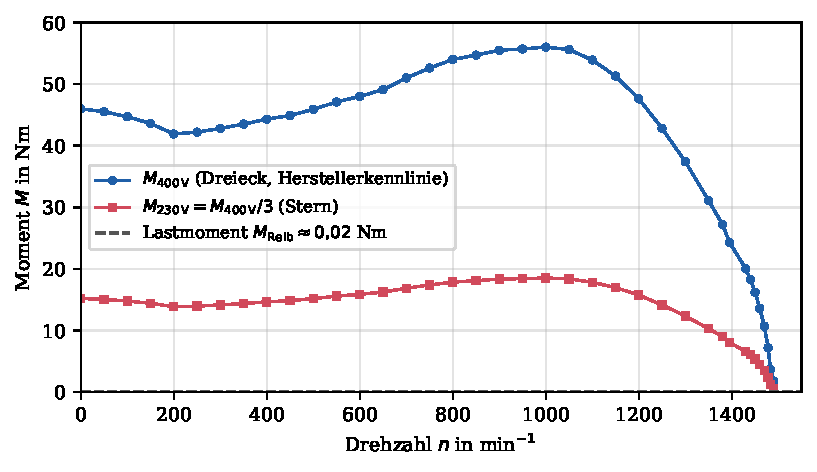
\includegraphics[width=0.88\textwidth]{v_kennlinie}
\caption{Motormoment über der Drehzahl im Dreieck (\SI{400}{V}) und im Stern
(\SI{230}{V} am Strang) sowie das Lastmoment durch Lagerreibung}
\label{fig:kennlinie}
\end{figure}

Die Zeit für jeden Drehzahlschritt folgt aus Gl.~\eqref{eq:dt}. Als Moment wird der
Mittelwert an den Intervallgrenzen verwendet, abzüglich des Reibmoments. Beispiel für den ersten Schritt
(\SIrange{0}{50}{\per\minute}, Moment am Intervallanfang wie in der Anleitung):
\[
  \Delta t = \frac{2\pi\cdot \SI{0,3745}{kg.m^2}\cdot \frac{50}{60}\,\si{\per\second}}{\SI{46}{Nm}}
  \approx \SI{\WdtBsp}{ms}.
\]
Die Summe aller Zeitschritte ergibt den Hochlaufverlauf $n(t)$
(Tab.~\ref{tab:hochlauf}, Abb.~\ref{fig:hochlauf}). Da das Motormoment kurz vor der
synchronen Drehzahl gegen null geht, wird die Integration bei
\SI{1480}{\per\minute} beendet.

{\small
\begin{longtable}{@{}c c c c c c c@{}}
\caption{Numerische Integration der Hochlaufzeit
($J=\SI{0,3745}{kg.m^2}$, $M$: Intervallmittelwert abzüglich Reibmoment)}
\label{tab:hochlauf}\\
\toprule
$n$-Intervall & $M_\Delta$ & $M_Y$ & $\Delta t_\Delta$ & $t_\Delta$ & $\Delta t_Y$ & $t_Y$\\
in \si{\per\minute} & in \si{Nm} & in \si{Nm} & in \si{ms} & in \si{s} & in \si{ms} & in \si{s}\\
\midrule
\endfirsthead
\toprule
$n$-Intervall & $M_\Delta$ & $M_Y$ & $\Delta t_\Delta$ & $t_\Delta$ & $\Delta t_Y$ & $t_Y$\\
\midrule
\endhead
\csname @@input\endcsname tabelle_hochlauf.tex 
\bottomrule
\end{longtable}
}

\begin{figure}[H]
\centering
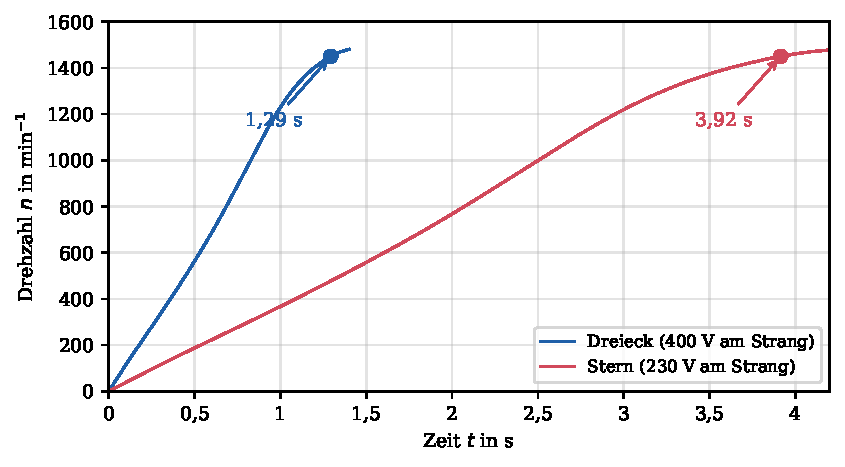
\includegraphics[width=0.88\textwidth]{v_hochlauf}
\caption{Berechneter Hochlauf (nicht normiert) für Dreieck- und Sternbetrieb}
\label{fig:hochlauf}
\end{figure}

\begin{table}[H]
\centering
\caption{Berechnete Hochlaufzeiten}
\label{tab:tH}
\begin{tabular}{@{}lccc@{}}
\toprule
Schaltung & bis \SI{1400}{\per\minute} & bis \SI{1450}{\per\minute} & bis \SI{1480}{\per\minute}\\
\midrule
Dreieck (\SI{400}{V}) & \SI{\WtHDA}{s} & \SI{\WtHDB}{s} & \SI{\WtHDC}{s}\\
Stern (\SI{230}{V})  & \SI{\WtHYA}{s} & \SI{\WtHYB}{s} & \SI{\WtHYC}{s}\\
\bottomrule
\end{tabular}
\end{table}
Im Stern ist das Moment auf ein Drittel reduziert. Die Hochlaufzeit verlängert sich deshalb genau
um den Faktor drei. \textbf{Umschaltzeitpunkt:} Die Maschine sollte im Stern bis knapp
unter die Nenndrehzahl hochlaufen. Nach der Rechnung ist das nach etwa
\SIrange{3,6}{3,9}{s} der Fall (\SIrange{1400}{1450}{\per\minute}).

% =====================================================================
\section{Messergebnisse und Auswertung: Anlaufverfahren}
% =====================================================================
Gemessen wurden Drehzahl, Effektivwerte von Spannung und Strom sowie Wirk- und
Blindleistung. In allen Diagrammen ist $t=0$ der Einschaltzeitpunkt. Die grau
hinterlegten Bereiche markieren die stromlose Umschaltpause von Stern auf Dreieck.

\subsection{Direkter Dreieckanlauf}
\begin{figure}[H]
\centering
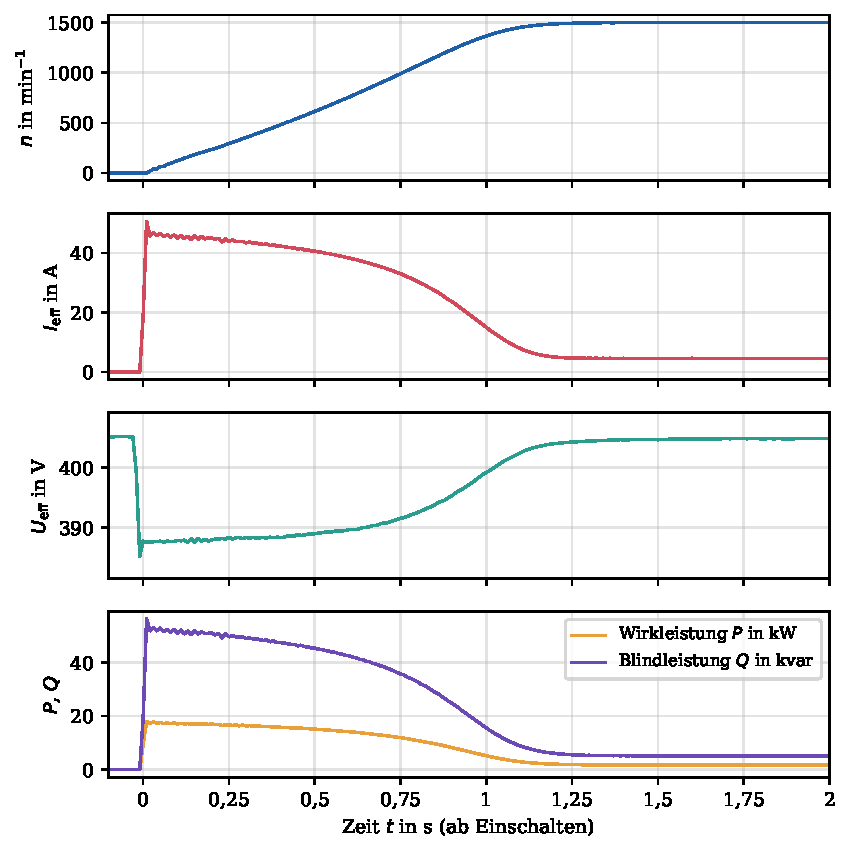
\includegraphics[width=0.86\textwidth]{a_direkt}
\caption{Direkter Dreieckanlauf: Drehzahl, Strom, Spannung und Leistungen}
\label{fig:direkt}
\end{figure}
Beim Einschalten springt der Strom auf \SI{\WdirektIeins}{A}, das sind etwa das
\WdirektIN-fache des Bemessungsstroms. Dieser Wert bleibt bis etwa \SI{1000}{\per\minute} nahezu
konstant und fällt erst nach dem Kippmoment auf den Leerlaufstrom von
\SI{\WdirektIend}{A}. Die Netzspannung bricht während des Hochlaufs von
\SI{\WdirektUnull}{V} auf \SI{\WdirektUeins}{V} ein (\SI{\WdirektdU}{\percent}).
Die Blindleistung ist mit \SI{\WdirektQeins}{var} rund dreimal so groß wie die
Wirkleistung (\SI{\WdirektPeins}{W}), daraus folgt $\cos\varphi\approx0{,}30$.
Nach \SI{\Wdirekttneunacht}{s} sind \SI{98}{\percent} der Enddrehzahl
(\SI{\Wdirektnend}{\per\minute}) erreicht.

\subsection{Stern-Dreieck-Anlauf, zu früh umgeschaltet}
\begin{figure}[H]
\centering
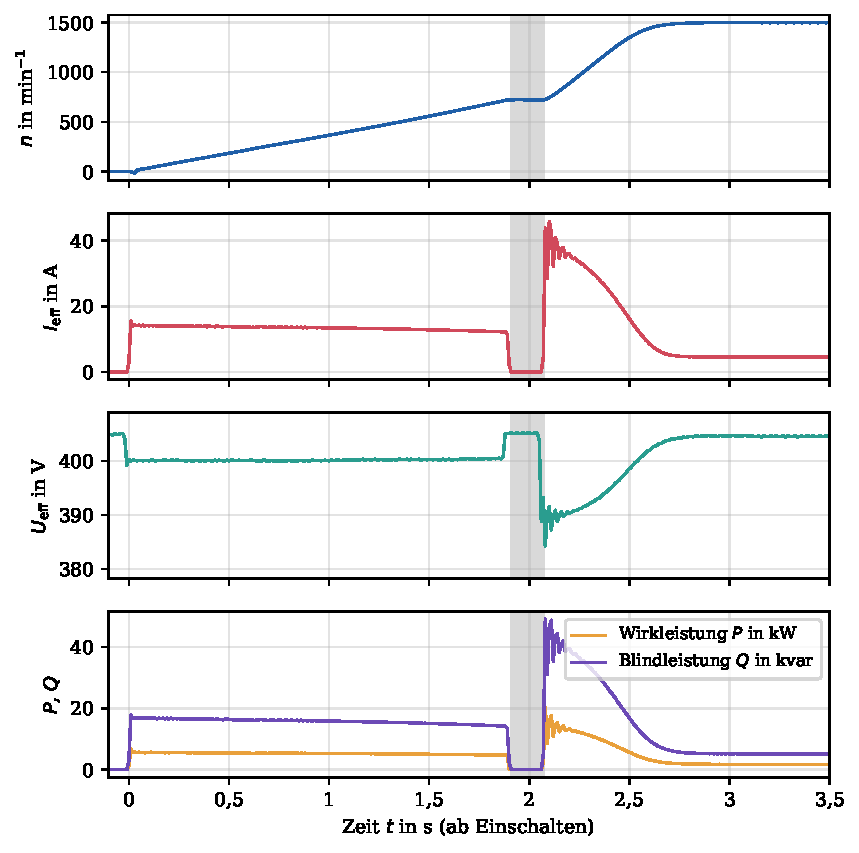
\includegraphics[width=0.86\textwidth]{a_frueh}
\caption{Stern-Dreieck-Anlauf mit zu früher Umschaltung}
\label{fig:frueh}
\end{figure}
Im Stern beträgt der Anlaufstrom nur \SI{\WfruehIeins}{A}, also etwa ein Drittel des Direktanlaufs.
Die Spannung bricht nur um \SI{\WfruehdU}{\percent} ein. Die Maschine beschleunigt
deutlich langsamer. Umgeschaltet wurde laut Messdaten nach
\SI{\Wfruehtum}{s} bei erst \SI{\Wfruehnum}{\per\minute} (also etwa bei der halben
Synchrondrehzahl). Die Umschaltpause dauerte \SI{\Wfruehpause}{s}.
Nach dem Umschalten entsteht ein zweiter Stromstoß von \SI{\WfruehIzwei}{A}
mit einem Spannungseinbruch auf \SI{\WfruehUzwei}{V} (\SI{\WfruehdUzwei}{\percent}).
Strom und Spannungseinbruch sind damit fast so groß wie beim direkten Dreieckanlauf.
Die Maschine läuft danach wie beim Direktanlauf mit hohem Strom weiter hoch, bis sie
nach insgesamt \SI{\Wfruehtneunacht}{s} die Enddrehzahl erreicht. Der Vorteil des
Stern-Dreieck-Anlaufs geht durch das zu frühe Umschalten weitgehend verloren.

\subsection{Stern-Dreieck-Anlauf, richtig umgeschaltet}
\begin{figure}[H]
\centering
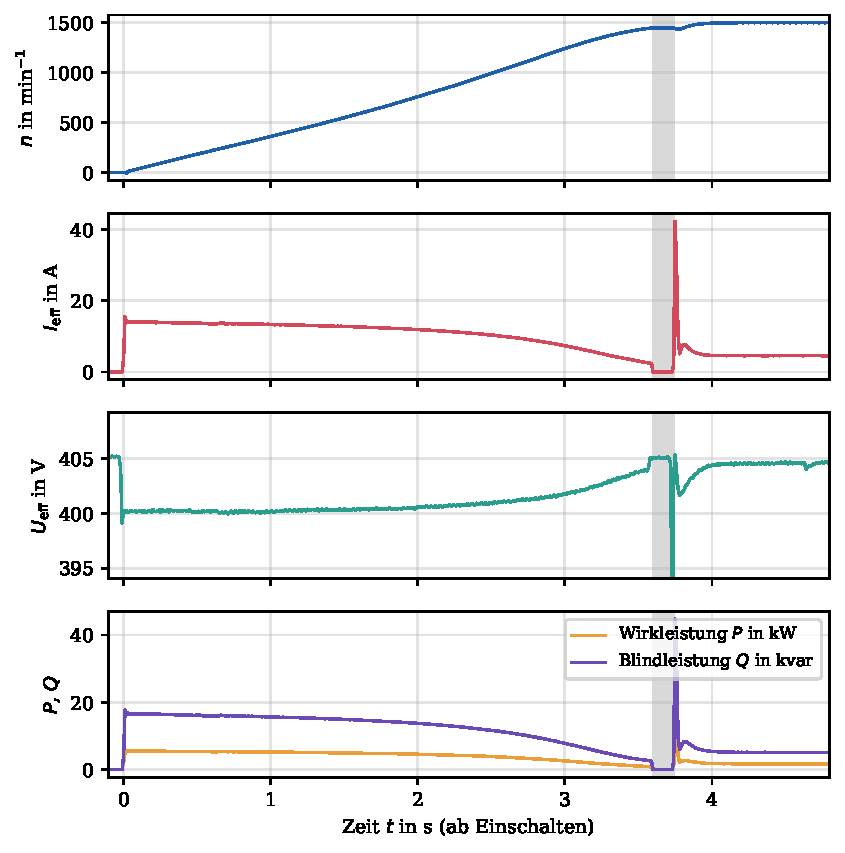
\includegraphics[width=0.86\textwidth]{a_richtig}
\caption{Stern-Dreieck-Anlauf mit Umschaltung zum berechneten Zeitpunkt}
\label{fig:richtig}
\end{figure}
Die Maschine läuft im Stern bis \SI{\Wrichtignum}{\per\minute} hoch
(Umschaltung nach \SI{\Wrichtigtum}{s}). Dieser Zeitpunkt stimmt gut mit der Rechnung
überein (Tab.~\ref{tab:tH}). Der Strom ist zu diesem Zeitpunkt bereits auf etwa
\SI{2,5}{A} abgesunken. Der Umschaltstromstoß ist mit \SI{\WrichtigIzwei}{A} nur sehr kurz
(ein bis zwei Messwerte, ca.\ \SI{20}{ms}), da die Maschine schon nahe der Nenndrehzahl ist.
Der Spannungseinbruch beim Umschalten beträgt nur \SI{\WrichtigdUzwei}{\percent}.
Die Spitze entsteht vor allem durch das Wiederzuschalten auf die noch magnetisierte
Maschine (Ausgleichsvorgang) und nicht durch einen erneuten Hochlauf.

\subsection{Stern-Dreieck-Anlauf, falsch verdrahtet}
\begin{figure}[H]
\centering
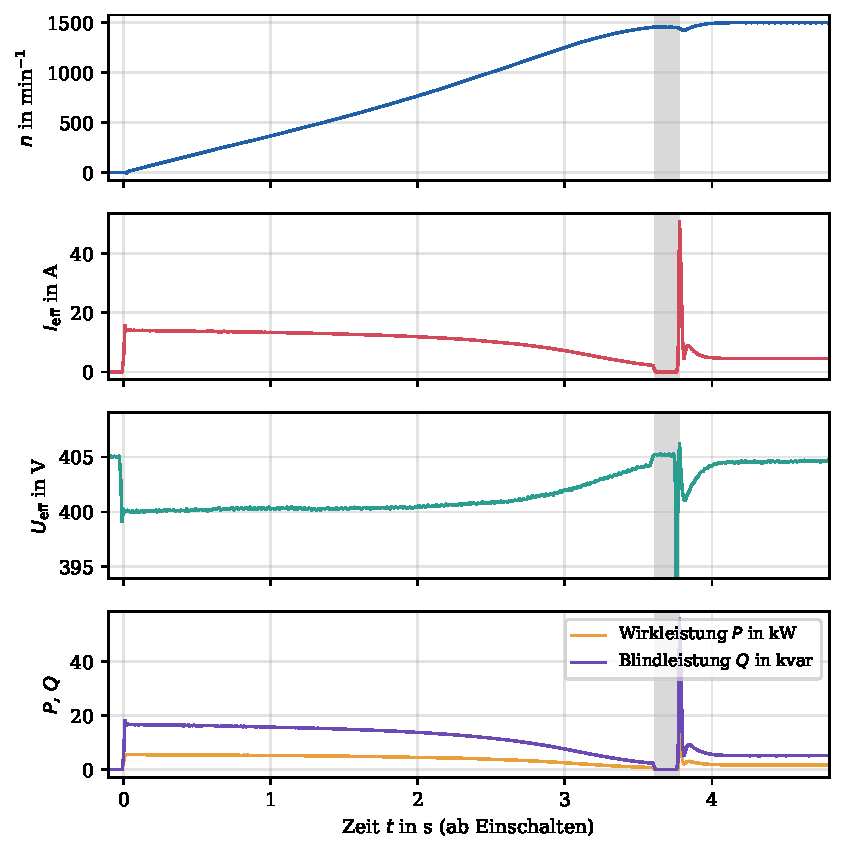
\includegraphics[width=0.86\textwidth]{a_falsch}
\caption{Stern-Dreieck-Anlauf mit falsch verdrahteter Dreieckschaltung}
\label{fig:falsch}
\end{figure}
Hochlauf im Stern und Umschaltzeitpunkt (\SI{\Wfalschtum}{s},
\SI{\Wfalschnum}{\per\minute}) entsprechen der richtigen Umschaltung. Der
Umschaltstromstoß ist mit \SI{\WfalschIzwei}{A} jedoch rund \SI{20}{\percent} größer,
und die Wirkleistungsspitze ist mit \SI{\WfalschPzwei}{W} fast doppelt so hoch wie
bei richtiger Verdrahtung (\SI{\WrichtigPzwei}{W}). Außerdem fällt die
Drehzahl nach dem Umschalten kurz um ca.\ \SI{30}{\per\minute} ab (richtig verdrahtet:
ca.\ \SI{10}{\per\minute}). Die Maschine wird beim Umschalten also kurz
abgebremst.

Erklärung: Beim Umschalten springen die Strangspannungen um \SI{30}{\degree}. Die
Richtung dieses Phasensprungs hängt davon ab, wie die Wicklungsenden
U2, V2, W2 im Dreieck an die Außenleiter angeschlossen sind. Während der kurzen
Umschaltpause ist der Läufer noch magnetisiert und induziert eine Restspannung, die
der Netzspannung nacheilt. Bei richtiger Zuordnung ist die Phasendifferenz zwischen
Netzspannung und Restspannung klein. Bei vertauschter Zuordnung ist sie
größer, daher entstehen ein größerer Ausgleichsstrom und ein kurzes Bremsmoment
(Drehzahleinbruch).

\subsection{Vergleich der Anlaufverfahren}
\begin{figure}[H]
\centering
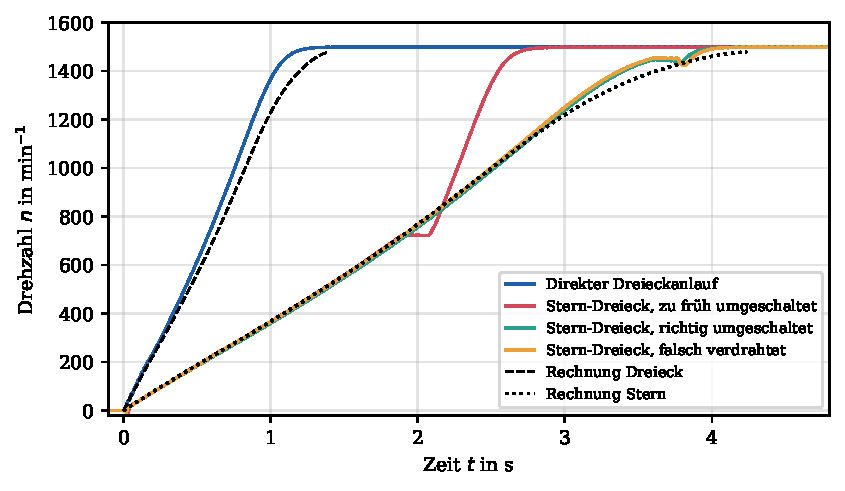
\includegraphics[width=0.88\textwidth]{a_vergleich_n}
\caption{Gemessene Drehzahlverläufe im Vergleich mit der Rechnung aus der Vorbereitung}
\label{fig:vergl_n}
\end{figure}
\begin{figure}[H]
\centering
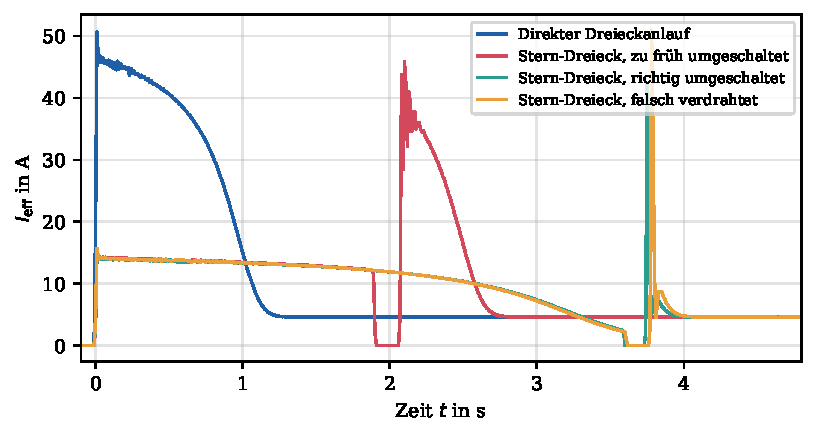
\includegraphics[width=0.88\textwidth]{a_vergleich_I}
\caption{Stromverläufe der Anlaufverfahren im Vergleich}
\label{fig:vergl_I}
\end{figure}

\begin{table}[H]
\centering
\caption{Kennwerte der Anlaufverfahren ($I_1$, $U_1$: Einschaltmoment;
$I_2$, $U_2$: nach dem Umschalten; $t_{98}$: Zeit bis \SI{98}{\percent} der Enddrehzahl;
$E$: aufgenommene Wirkenergie bis $t_{98}$)}
\label{tab:anlauf}
\small
\begin{tabular}{@{}l c c c c c c c@{}}
\toprule
Verfahren & $I_1$ & $U_1$ & $t_\mathrm{um}$ / $n_\mathrm{um}$ & $I_2$ & $U_2$ & $t_{98}$ & $E$\\
 & in A & in V & in s / \si{\per\minute} & in A & in V & in s & in kJ\\
\midrule
Direkt Dreieck & \WdirektIeins & \WdirektUeins & -- & -- & -- & \Wdirekttneunacht & 14,5\\
Y-$\Delta$ zu früh & \WfruehIeins & \WfruehUeins & \Wfruehtum{} / \Wfruehnum & \WfruehIzwei & \WfruehUzwei & \Wfruehtneunacht & 15,4\\
Y-$\Delta$ richtig & \WrichtigIeins & \WrichtigUeins & \Wrichtigtum{} / \Wrichtignum & \WrichtigIzwei & \WrichtigUzwei & \Wrichtigtneunacht & 15,8\\
Y-$\Delta$ falsch verdr. & \WfalschIeins & \WfalschUeins & \Wfalschtum{} / \Wfalschnum & \WfalschIzwei & \WfalschUzwei & \Wfalschtneunacht & 15,8\\
\bottomrule
\end{tabular}
\end{table}
Bei allen Verfahren liegt die Netzspannung vor dem Einschalten bei \SI{\WdirektUnull}{V}. Im
stationären Leerlauf nimmt die Maschine etwa \SI{\WrichtigIend}{A}, \SI{\WrichtigPend}{W} und
\SI{\WrichtigQend}{var} auf.
Das Verhältnis der Anlaufströme Dreieck/Stern beträgt
$\WdirektIeins/\WrichtigIeins \approx 3{,}3$ und bestätigt damit Gl.~\eqref{eq:stern}.

Die aufgenommene Wirkenergie ist bei allen Verfahren ähnlich. In der Schwungmasse
sind am Ende nur $E_\mathrm{kin}=\tfrac12 J\omega^2 \approx \SI{4,6}{kJ}$ gespeichert.
Beim Hochlauf einer ASM entsteht im Läufer zusätzlich eine Verlustenergie in
derselben Größe wie $E_\mathrm{kin}$. Dazu kommen Ständer- und Eisenverluste. Der Stern-Dreieck-Anlauf
senkt also die Strom\emph{spitzen}, aber nicht die Energie, die während des Hochlaufs umgesetzt wird.

\begin{antwort}{Frage: Wodurch entsteht der Spannungseinbruch in den Schaltmomenten, und wie kann er verringert werden?}
Der hohe, überwiegend induktive Einschaltstrom ($\cos\varphi\approx0{,}3$) fließt über die
Kurzschlussimpedanz von Transformator und Zuleitungen. Nach Gl.~\eqref{eq:kapp} liegt
der Spannungsabfall an $X_k$ dann nahezu in Phase mit der Netzspannung. Die Spannung an
den Motorklemmen sinkt daher deutlich: beim Direktanlauf um \SI{\WdirektdU}{\percent},
bei zu frühem Umschalten um \SI{\WfruehdUzwei}{\percent}, im Stern nur um \SI{\WrichtigdU}{\percent}.
Die kurzen Spannungsspitzen nach unten direkt beim Schalten entstehen
zusätzlich durch Ausgleichsvorgänge (Gleichanteile im Strom, Kontaktprellen).

\textbf{Maßnahmen:} kleinerer Anlaufstrom durch Stern-Dreieck-Anlauf mit
\emph{richtigem} Umschaltzeitpunkt und richtiger Verdrahtung, Sanftanlasser
(Drehstromsteller), Frequenzumrichter, Anlasstransformator, bei Schleifringläufern
Anlasswiderstände. Auf der Netzseite helfen ein leistungsstärkerer Transformator mit kleiner
Kurzschlussspannung $u_k$, größere Leiterquerschnitte und kürzere Leitungen
(kleineres $Z_k$) sowie Blindleistungskompensation.
\end{antwort}

\subsection{Vergleich berechnete und gemessene Hochlaufzeit}
\begin{table}[H]
\centering
\caption{Vergleich der Hochlaufzeiten (Zeit bis \SI{1450}{\per\minute})}
\label{tab:vergl_tH}
\begin{tabular}{@{}lccc@{}}
\toprule
Schaltung & berechnet & gemessen & Abweichung\\
\midrule
Dreieck (direkt) & \SI{\WtHDB}{s} & \SI{\Wdirektteinsvierfuenfnull}{s} & ca.\ \SI{-15}{\percent}\\
Stern (bis zur Umschaltung bei ca.\ \SI{1443}{\per\minute}) & \SI{\WtHYum}{s} & \SI{\Wrichtigtum}{s} & ca.\ \SI{-7}{\percent}\\
\bottomrule
\end{tabular}
\end{table}

\begin{antwort}{Frage: Vergleich der berechneten mit der gemessenen Hochlaufzeit}
Die gemessenen Hochlaufzeiten sind etwas kürzer als die berechneten
(Dreieck ca.\ \SI{15}{\percent}, Stern ca.\ \SI{7}{\percent}). Die Rechnung gibt den Verlauf
aber gut wieder (Abb.~\ref{fig:vergl_n}): Sattel bei niedriger Drehzahl,
größte Beschleunigung im Bereich des Kippmoments, starkes Abflachen kurz vor der
synchronen Drehzahl. Gründe für die Abweichung:
\begin{itemize}
\item Die Herstellerkennlinie ist ein typischer bzw.\ garantierter Mindestverlauf, die reale Maschine
      hat im Versuch ein größeres Moment (siehe Abschnitt~\ref{sec:mb}).
\item Die Netzspannung lag bei \SI{405}{V} statt \SI{400}{V} (+\SI{2,5}{\percent} Moment).
\item Die Kennlinie wurde aus einem Diagramm abgelesen (Ablesefehler).
\item Die Anleitung gibt mit \SI{0,3745}{kg.m^2} ein etwas größeres $J$ vor.
\item Die Rechnung endet bei einer festen Enddrehzahl. Wo genau „Hochlauf beendet“ ist, lässt sich
      kurz vor der Synchrondrehzahl schwer festlegen.
\end{itemize}
Für die Wahl des Umschaltzeitpunkts ist die Rechnung gut geeignet. Die zu frühe
Umschaltung nach \SI{\Wfruehtum}{s} lag deutlich unter der berechneten Zeit von ca.\ \SI{3,6}{s}.
\end{antwort}

\subsection{Beschleunigungsmoment aus der Drehzahländerung}
\label{sec:mb}
Aus dem gemessenen Drehzahlverlauf wird mit der Bewegungsgleichung das
Beschleunigungsmoment berechnet:
\begin{equation}
  M_\mathrm B(t) = J_\mathrm{Stahl}\cdot 2\pi\,\frac{\mathrm dn}{\mathrm dt},
  \qquad J_\mathrm{Stahl} = \tfrac12\cdot\SI{32,99}{kg}\cdot(\SI{0,15}{m})^2 = \SI{\WJStahl}{kg.m^2}.
\end{equation}
Da das Drehzahlsignal verrauscht ist, wurde es vor dem Ableiten mit einem
Savitzky-Golay-Filter (15 Werte $\hat=$ \SI{150}{ms}, Polynomgrad 2) geglättet.

\begin{figure}[H]
\centering
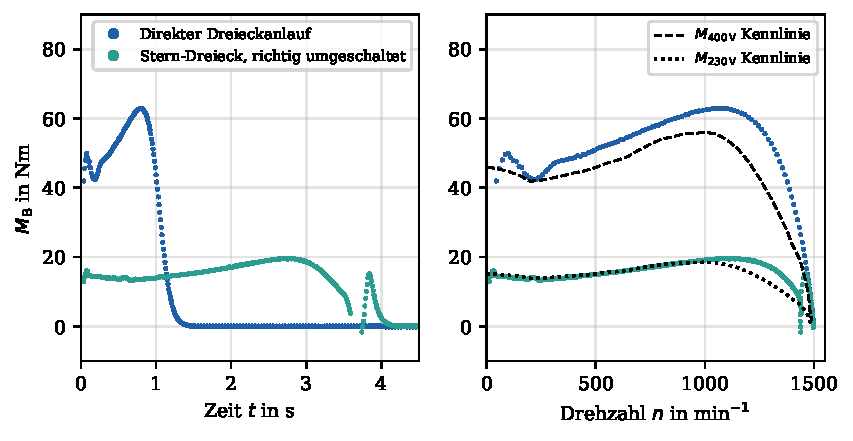
\includegraphics[width=\textwidth]{a_moment}
\caption{Beschleunigungsmoment aus der gemessenen Drehzahländerung, links über der Zeit,
rechts über der Drehzahl im Vergleich mit der Kennlinie aus der Vorbereitung}
\label{fig:moment}
\end{figure}

Das gemessene Moment zeigt die typische Form der ASM-Kennlinie: Anzugsmoment,
Sattelmoment bei ca.\ \SI{200}{\per\minute}, Kippmoment bei ca.\ \SI{1000}{\per\minute},
danach starker Abfall bis zur Leerlaufdrehzahl. Im Bereich
\SIrange{200}{1000}{\per\minute} beträgt das mittlere Beschleunigungsmoment
\begin{itemize}
\item im Dreieck \SI{\WdirektMBmittel}{Nm} (Kennlinie: \SI{\WMkennDmittel}{Nm}) und
\item im Stern \SI{\WrichtigMBmittel}{Nm} (Kennlinie: \SI{\WMkennYmittel}{Nm}).
\end{itemize}
Im Stern stimmen Messung und Kennlinie gut überein. Im Dreieck liegt das gemessene Moment um
etwa \SI{8}{\percent} über der Kennlinie, besonders im Kippbereich (ca.\ \SI{62}{Nm} gegenüber
\SI{56}{Nm}). Das erklärt die kürzere gemessene Hochlaufzeit. Das
Kippmoment beträgt etwa das Dreifache des Bemessungsmoments. Beim Umschalten
(Stern-Dreieck) ist die kurze Momentenspitze zu sehen.

% =====================================================================
\section{Messergebnisse und Auswertung: Bremsverfahren}
% =====================================================================
Die Bremsversuche wurden an der umrichtergespeisten ASM mit Aluminium-Schwungscheibe
bei einer Ausgangsdrehzahl von ca.\ \SI{1800}{\per\minute} (\SI{60}{Hz}) durchgeführt.
$t=0$ ist jeweils der Bremsbefehl. Die kinetische Energie der Schwungscheibe beträgt
\[
  E_\mathrm{kin} = \tfrac12 J_\mathrm{Alu}\,\omega^2
  = \tfrac12\cdot\SI{\WJAlu}{kg.m^2}\cdot\left(2\pi\cdot 30\,\si{\per\second}\right)^2
  \approx \SI{\WEkin}{J}.
\]
Das Bremsmoment wird analog zu Abschnitt~\ref{sec:mb} berechnet:
$M_\mathrm{Br} = -J_\mathrm{Alu}\cdot2\pi\,\mathrm dn/\mathrm dt$
(Läuferträgheit vernachlässigt).

\subsection{Drehzahlverläufe im Überblick}
\begin{figure}[H]
\centering
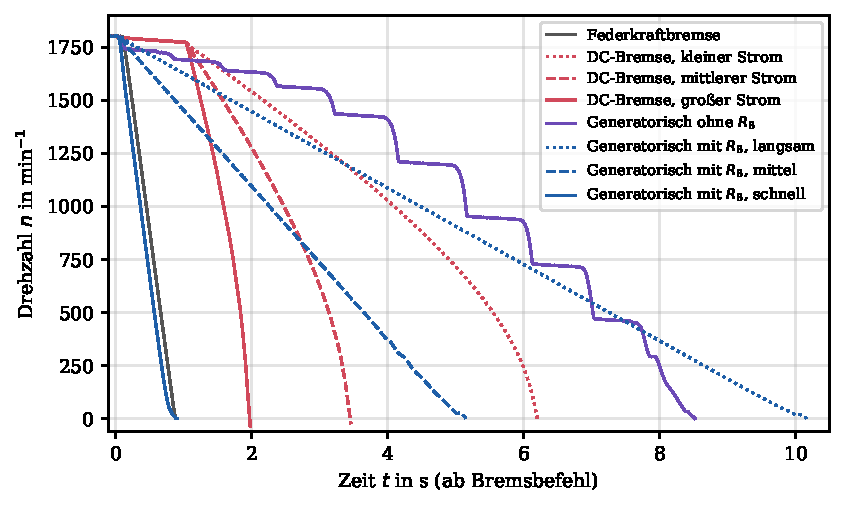
\includegraphics[width=0.9\textwidth]{b_vergleich_n}
\caption{Drehzahlverläufe aller Bremsverfahren}
\label{fig:b_n}
\end{figure}

\begin{table}[H]
\centering
\caption{Kennwerte der Bremsverfahren ($t_\mathrm B$: Zeit vom Bremsbefehl bis
$n<\SI{10}{\per\minute}$; $\bar a$: mittlere Verzögerung; $\bar M$: mittleres Bremsmoment während
der wirksamen Bremsphase; $E_\mathrm{RB}$: Energie im Bremswiderstand)}
\label{tab:bremsen}
\small
\begin{tabular}{@{}l c c c c c c@{}}
\toprule
Verfahren & $t_\mathrm B$ & $\bar a$ & $\bar M$ & $M_\mathrm{max}$ & $U_\mathrm{ZK,max}$ & $E_\mathrm{RB}$\\
 & in s & in \si{\per\minute\per\second} & in Nm & in Nm & in V & in J\\
\midrule
\csname @@input\endcsname tabelle_bremsen.tex 
\bottomrule
\end{tabular}
\end{table}

\subsection{Federkraftbremse}
\begin{figure}[H]
\centering
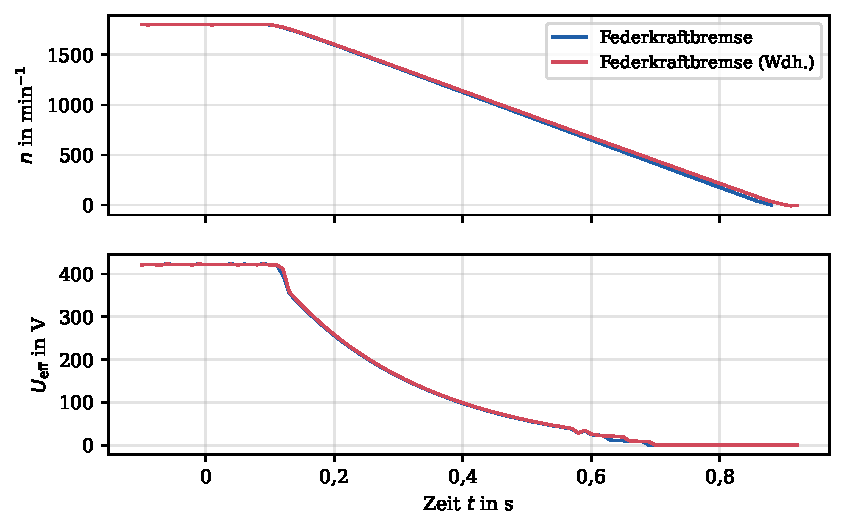
\includegraphics[width=0.86\textwidth]{b_feder}
\caption{Federkraftbremse (zwei Messungen)}
\label{fig:feder}
\end{figure}
Beim Bremsbefehl werden der Umrichter und die Bremsspule gleichzeitig abgeschaltet. Nach einer
Einfallzeit von ca.\ \SI{\Wfederts}{s} (Abbau des Magnetfelds der Lüftspule, Weg der
Ankerscheibe) setzt die Bremse ein. Die Drehzahl nimmt danach \emph{linear} ab, das
Bremsmoment ist also nahezu konstant (Coulomb'sche Reibung, unabhängig von der Drehzahl).
Es beträgt ca.\ \SI{\WfederMmit}{Nm}, das ist etwa das 1,5-fache Bemessungsmoment. Die Maschine
steht nach \SI{\WfedertB}{s}. Die Wiederholungsmessung bestätigt das Ergebnis
(\SI{\WfedernulltB}{s}, \SI{\WfedernullMmit}{Nm}). Die Klemmenspannung zeigt nur noch
die abklingende Restspannung des Läufers.

\subsection{Gleichstrombremsung (DC-Bremse)}
\begin{figure}[H]
\centering
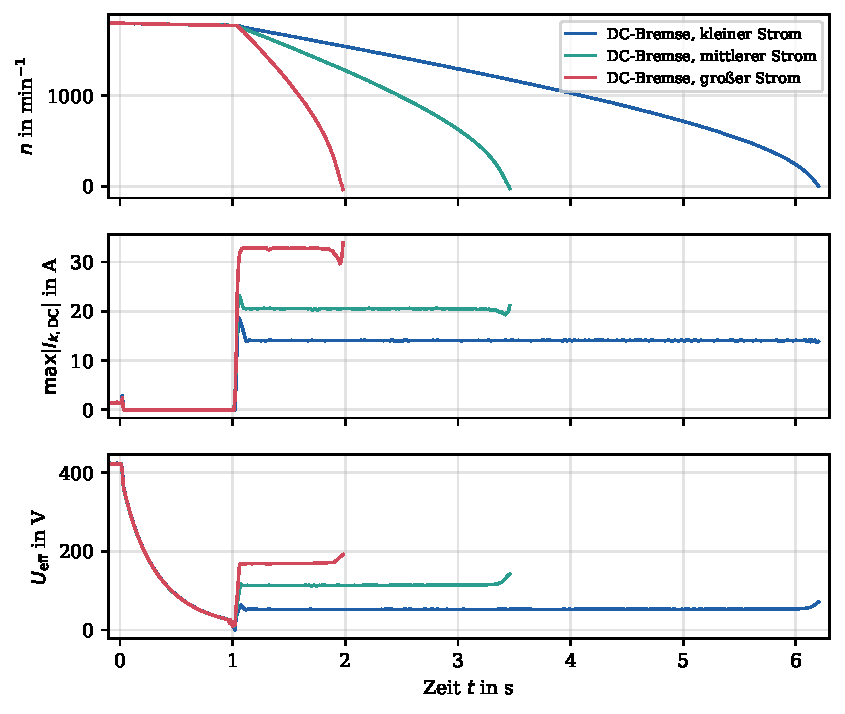
\includegraphics[width=0.86\textwidth]{b_dc}
\caption{Gleichstrombremsung mit drei verschiedenen Bremsströmen}
\label{fig:dc}
\end{figure}
Nach dem Bremsbefehl sperrt der Umrichter zunächst die Pulse. Die Maschine trudelt
ca.\ \SI{1}{s} aus, bis die Restspannung des Läufers abgeklungen ist (Entmagnetisierungszeit).
Erst dann wird der Gleichstrom eingespeist (ab $t\approx\SI{1,03}{s}$). Gemessen wurden:

\begin{table}[H]
\centering
\caption{Ergebnisse der Gleichstrombremsung}
\label{tab:dc}
\begin{tabular}{@{}lcccc@{}}
\toprule
Einstellung & $I_\mathrm{DC}$ & Bremsdauer ab DC-Einspeisung & $\bar M$ & $\bar M/\bar M_\mathrm{klein}$\\
\midrule
kleiner Strom & \SI{\WdclIdcB}{A} & \SI{\WdcltnachI}{s} & \SI{\WdclMmit}{Nm} & 1,0\\
mittlerer Strom & \SI{\WdcmIdcB}{A} & \SI{\WdcmtnachI}{s} & \SI{\WdcmMmit}{Nm} & 2,1\\
großer Strom & \SI{\WdcsIdcB}{A} & \SI{\WdcstnachI}{s} & \SI{\WdcsMmit}{Nm} & 5,5\\
\bottomrule
\end{tabular}
\end{table}

Das mittlere Bremsmoment wächst quadratisch mit dem Gleichstrom:
$(20{,}5/14{,}1)^2 = 2{,}1$ und $(32{,}8/14{,}1)^2 = 5{,}4$, das stimmt mit den
gemessenen Verhältnissen überein. Über den Bremsstrom lässt sich die Bremszeit also gezielt einstellen.
Das Bremsmoment ist bei hoher Drehzahl klein und \emph{steigt zu kleinen Drehzahlen hin
stark an} (Abb.~\ref{fig:b_moment}). Die Drehzahlkurve wird deshalb zum Ende hin immer steiler.
Der Grund: Die Läuferfrequenz entspricht bei der DC-Bremse der Drehzahl. Bei niedriger
Drehzahl ist die Läuferreaktanz klein und der Läuferstrom liegt besser in Phase mit
dem Feld. Das Momentenmaximum liegt daher bei kleiner Drehzahl (ähnlich wie ein Kippmoment).
Im Stillstand fällt das Moment auf null. Ein Haltemoment gibt es nicht: Beim großen
Strom schwingt die Drehzahl am Ende sogar kurz ins Negative. Die gesamte kinetische
Energie und zusätzlich die Stromwärme $I_\mathrm{DC}^2R$ werden \emph{im Motor} in Wärme umgesetzt.
Die Zwischenkreisspannung bleibt unverändert bei ca.\ \SI{580}{V}.

\subsection{Generatorisches Bremsen ohne Bremswiderstand}
\begin{figure}[H]
\centering
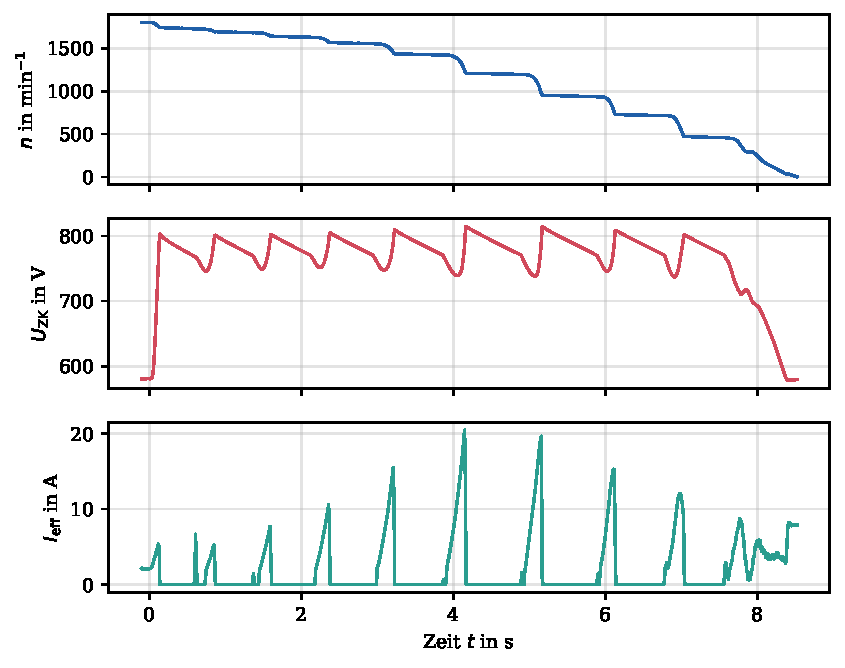
\includegraphics[width=0.86\textwidth]{b_gen0}
\caption{Generatorisches Bremsen ohne Bremswiderstand: Drehzahl,
Zwischenkreisspannung und Motorstrom}
\label{fig:gen0}
\end{figure}
Sobald der Umrichter die Frequenz absenkt, speist die Maschine Energie in den
Zwischenkreis zurück. $U_\mathrm{ZK}$ steigt von \SI{580}{V} auf bis zu
\SI{\WgenohneUzkmax}{V}. Ab ca.\ \SI{790}{V} sperrt der Umrichter die Pulse
(Überspannungsschutz bzw.\ Überspannungsregler). Der Motorstrom ist deshalb die meiste Zeit
null, und die Maschine trudelt fast ungebremst. Erst wenn $U_\mathrm{ZK}$ über
die Entladewiderstände bzw.\ die Eigenverluste wieder gesunken ist, folgt der nächste kurze
Bremsimpuls. Der Drehzahlverlauf ist daher stufenförmig, und die Bremszeit verlängert
sich auf \SI{\WgenohnetB}{s} (mittleres Bremsmoment nur \SI{\WgenohneMmit}{Nm}).

\subsection{Generatorisches Bremsen mit Bremswiderstand}
\begin{figure}[H]
\centering
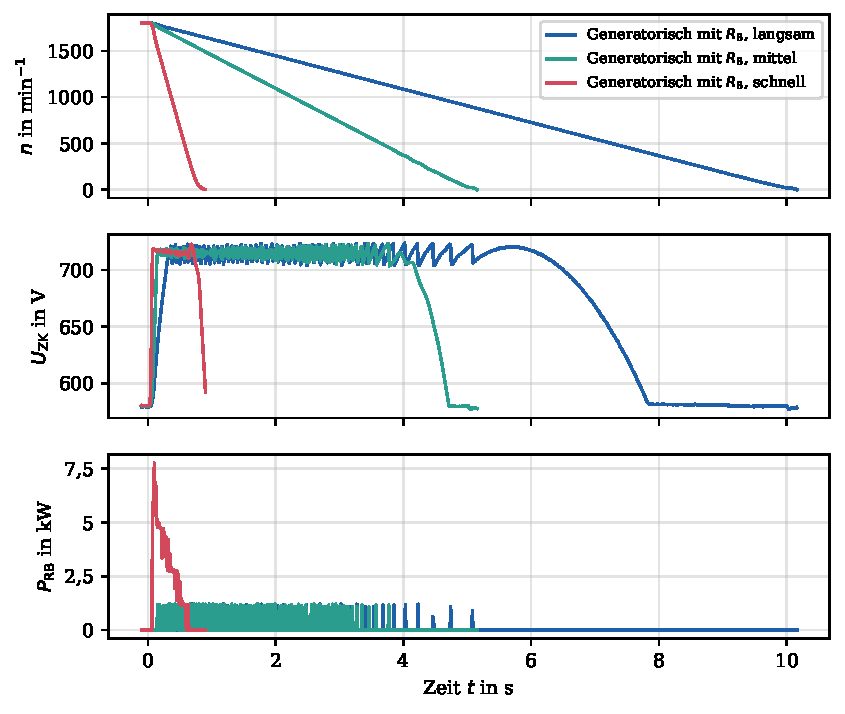
\includegraphics[width=0.86\textwidth]{b_gen}
\caption{Generatorisches Bremsen mit Bremswiderstand bei drei Rampenzeiten}
\label{fig:gen}
\end{figure}
Mit Bremswiderstand begrenzt der Brems-Chopper die Zwischenkreisspannung auf ca.\
\SIrange{715}{724}{V}. Die Maschine folgt der eingestellten Rampe genau:
Die Drehzahl nimmt linear ab und das Bremsmoment ist konstant
(langsam: \SI{\WgenltB}{s}, \SI{\WgenlMmit}{Nm}; mittel: \SI{\WgenmtB}{s}, \SI{\WgenmMmit}{Nm};
schnell: \SI{\WgenstB}{s}, \SI{\WgensMmit}{Nm}).
Bei der langsamen Rampe decken die Verluste in Motor und Umrichter einen großen Teil
der Bremsleistung, der Chopper schaltet nur selten ($E_\mathrm{RB}=\SI{\WgenlErb}{J}$).
Bei der schnellen Rampe nimmt der Widerstand Spitzenleistungen bis \SI{\WPRbmax}{W}
auf. Aus Zwischenkreisspannung, Effektiv- und Mittelwert des Widerstandsstroms ergibt sich
ein Bremswiderstand von ca.\ $R_\mathrm B\approx\SI{\WRb}{\ohm}$.

\textbf{Energiebilanz (schnell):} Im Bremswiderstand werden
$E_\mathrm{RB}=\int P_\mathrm{RB}\,\mathrm dt\approx\SI{\WgensErb}{J}$ umgesetzt, das sind ca.\
\SI{\WgensErbAnteil}{\percent} der kinetischen Energie der Scheibe (\SI{\WEkin}{J}). Den Rest
decken die Verluste in Motor und Umrichter sowie die Reibung. Der Läufer selbst
speichert ebenfalls Energie, die hier nicht berücksichtigt ist.

\subsection{Bremsmomente}
\begin{figure}[H]
\centering
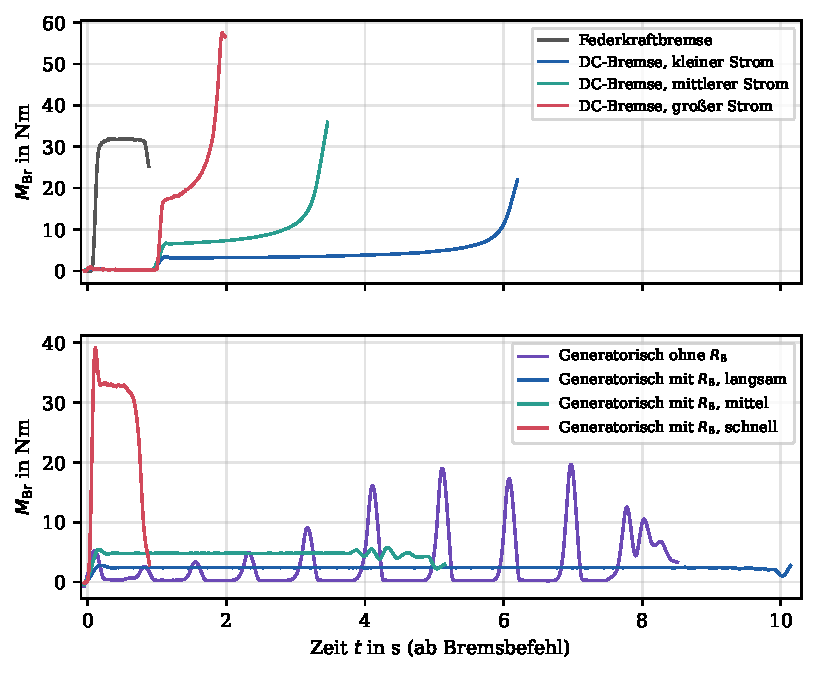
\includegraphics[width=0.9\textwidth]{b_moment}
\caption{Bremsmoment aus der gemessenen Drehzahländerung ($J_\mathrm{Alu}=\SI{\WJAlu}{kg.m^2}$),
oben: Federkraft- und DC-Bremse, unten: generatorisches Bremsen}
\label{fig:b_moment}
\end{figure}
\begin{figure}[H]
\centering
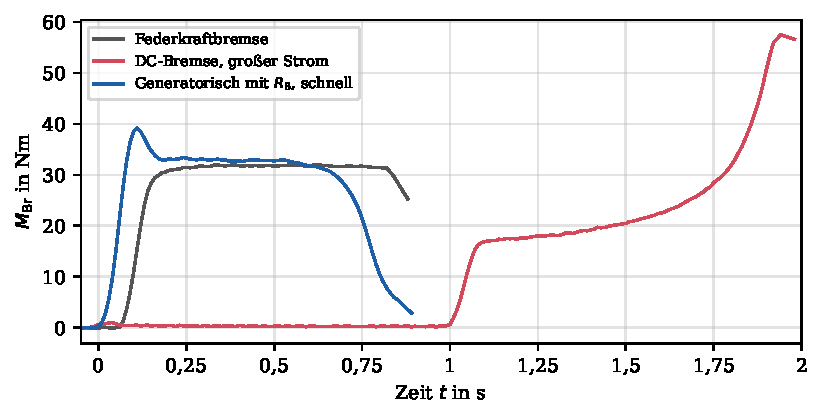
\includegraphics[width=0.9\textwidth]{b_moment_zoom}
\caption{Bremsmomente der drei schnellsten Verfahren im Vergleich}
\label{fig:b_moment_zoom}
\end{figure}
Die Verläufe zeigen die Eigenschaften der Verfahren deutlich: Federkraftbremse und
generatorisches Bremsen mit Rampe haben ein nahezu konstantes Moment. Bei der DC-Bremse steigt
das Moment zum Stillstand hin an. Beim generatorischen Bremsen ohne Widerstand treten nur
einzelne Momentimpulse auf. Die Spitzen am Anfang und am Ende einer Bremsung entstehen
teilweise durch die Glättung der Drehzahl beim Ableiten.

\begin{antwort}{Frage: Warum gibt es so große Unterschiede in der Verzögerungszeit beim generatorischen Bremsen mit und ohne Bremswiderstand?}
Beim generatorischen Bremsen fließt die kinetische Energie über den Wechselrichter in den
Zwischenkreis. Der Eingangsgleichrichter des Umrichters ist ein ungesteuerter Diodengleichrichter
und kann keine Energie ins Netz zurückspeisen. Ohne Bremswiderstand kann die Energie nur den
Zwischenkreiskondensator aufladen ($E=\tfrac12 C U^2$). Das reicht nur für einen kleinen Teil
der rund \SI{2,3}{kJ}. $U_\mathrm{ZK}$ erreicht nach kurzer Zeit die Überspannungsgrenze
(gemessen: \SI{\WgenohneUzkmax}{V}). Der Umrichter sperrt die Pulse oder verlängert die
Rampe. Die Maschine trudelt dann fast ungebremst, und die Bremszeit steigt auf
\SI{\WgenohnetB}{s}.

Mit Bremswiderstand schaltet der Brems-Chopper ab ca.\ \SI{720}{V} den Widerstand zu und
wandelt die Energie in Wärme um. $U_\mathrm{ZK}$ bleibt begrenzt, der Umrichter kann das
volle Bremsmoment aufbringen und die Rampe einhalten (\SI{\WgenstB}{s} bei schneller Rampe).
Alternativ könnte ein rückspeisefähiger Umrichter (Active Front End) die Energie ins Netz zurückgeben.
\end{antwort}

\begin{antwort}{Frage: Welches Verfahren kann als Not-Halt verwendet werden?}
Als Not-Halt ist nur die \textbf{Federkraftbremse} uneingeschränkt geeignet:
\begin{itemize}
\item Sie arbeitet nach dem \emph{Ruhestromprinzip}. Bei Netzausfall, Not-Aus,
      Kabelbruch oder Umrichterfehler fällt sie selbstständig ein (ausfallsicher).
\item Sie braucht keine Energie und keine funktionierende Elektronik.
\item Sie bremst mit konstantem, hohem Moment (\SI{\WfederMmit}{Nm}, Stillstand nach
      \SI{\WfedertB}{s}) und \emph{hält} die Last im Stillstand (wichtig z.\,B.\ bei
      Hubwerken).
\end{itemize}
DC-Bremse und generatorisches Bremsen hängen vom Netz und vom fehlerfreien Umrichter ab. Bei
Netzausfall wirken sie nicht. Die DC-Bremse hat außerdem kein Haltemoment, und ohne
Bremswiderstand ist das generatorische Bremsen sehr langsam. Das generatorische Bremsen mit
Bremswiderstand ist zwar ähnlich schnell, aber nicht ausfallsicher. In der Praxis kombiniert man
die Verfahren (Stopp-Kategorie~1 nach EN~60204-1): Zuerst wird gesteuert generatorisch gebremst,
danach fällt die mechanische Bremse ein und die Energie wird abgeschaltet.
\end{antwort}

% =====================================================================
\section{Zusammenfassung}
% =====================================================================
\begin{itemize}
\item Der \textbf{direkte Dreieckanlauf} ist am schnellsten (\SI{\Wdirekttneunacht}{s}), belastet das
      Netz aber mit dem \WdirektIN-fachen Bemessungsstrom und einem Spannungseinbruch von
      \SI{\WdirektdU}{\percent}.
\item Der \textbf{Stern-Dreieck-Anlauf} senkt Anlaufstrom und Moment auf ein Drittel. Er
      bringt nur Vorteile, wenn erst nahe der Nenndrehzahl umgeschaltet wird. Bei zu früher
      Umschaltung (\SI{\Wfruehnum}{\per\minute}) entsteht ein zweiter Stromstoß von
      \SI{\WfruehIzwei}{A}. Eine falsche Verdrahtung vergrößert den Umschaltstoß und bremst
      die Maschine kurz ab.
\item Die \textbf{berechnete Hochlaufzeit} stimmt in Verlauf und Größenordnung mit der
      Messung überein. Die Messung ist \SIrange{7}{15}{\percent} schneller, weil die reale
      Maschine ein größeres Moment hat.
\item Die \textbf{Federkraftbremse} bremst schnell mit konstantem Moment, ist ausfallsicher
      und daher für den Not-Halt geeignet.
\item Bei der \textbf{DC-Bremse} wächst das Bremsmoment mit $I_\mathrm{DC}^2$ und steigt zu kleinen
      Drehzahlen hin an. Es gibt kein Haltemoment, und der Motor wird stark erwärmt.
\item \textbf{Generatorisches Bremsen} braucht einen Bremswiderstand (oder Rückspeisung).
      Ohne ihn begrenzt die Zwischenkreis-Überspannung die Bremsung (\SI{\WgenohnetB}{s} statt
      \SI{\WgenstB}{s}).
\end{itemize}

% =====================================================================
\section{Risikobewertung}
% =====================================================================
\begin{itemize}
\item Die rotierende Schwungmasse ist eine mechanische Gefahr. Getragen wird nur eng
      anliegende Kleidung, lange Haare werden zusammengebunden oder bedeckt.
\item Durch den Messaufbau besteht die Gefahr eines elektrischen Schlags. Der Aufbau war vorverdrahtet
      und wurde nur vom Laborbetreuer bedient. Der Versuch wurde über einen Trenntransformator
      (galvanische Trennung) betrieben.
\item Bremswiderstand und Motor können sich bei häufigem Bremsen stark erwärmen
      (Verbrennungsgefahr).
\end{itemize}

% =====================================================================
\sloppy
\section*{Quellen}
\addcontentsline{toc}{section}{Quellen}
% =====================================================================
\begin{enumerate}[label={[\arabic*]}]
\item Ostfalia Hochschule, Labor für elektrische Antriebe: Versuchsanleitung V9
      „Anlauf- und Bremsverfahren“, Version 0.9, 08.10.2026.
\item Siemens AG: Aufbau Federkraftbremse, Bilddatenbank,
      \url{https://www.automation.siemens.com/bilddb}, Abruf 24.09.2024.
\item Lenze SE: Produktinformation Gleichstrombremsung,
      \url{https://www.lenze.com}, Abruf 24.09.2024.
\item K.-D.\ Tieste: Skript „Elektrische Antriebe“, Ostfalia Hochschule, WS 2024/25.
\end{enumerate}

\appendix
\section{Hinweise zur Auswertung}
Alle Diagramme und Kennwerte wurden mit dem Python-Skript
\texttt{auswertung/auswertung.py} aus den Original-CSV-Dateien erzeugt (NumPy, SciPy,
Matplotlib). Die Momente wurden aus der mit einem Savitzky-Golay-Filter geglätteten Drehzahl
abgeleitet. Die Leistungsmessgeräte liefern \SI{10}{ms}-Effektivwerte. Sehr kurze
Stromspitzen (z.\,B.\ die Einschaltspitze) werden dadurch teilweise unterschätzt.
\end{document}
